\documentclass[11pt, a4paper]{article}

\usepackage[margin=2.3cm]{geometry}
\usepackage{amsmath, amssymb, amsthm, mathtools}
\usepackage{bm}
\usepackage{tikz}
\usetikzlibrary{positioning, arrows.meta, fit, backgrounds, calc}
\usepackage{booktabs}
\usepackage{enumitem}
\usepackage{microtype}
\usepackage{xcolor}
\usepackage{fontspec}
\setmonofont{JetBrainsMono Nerd Font}[Scale=MatchLowercase]
\usepackage[newfloat]{minted}
\usepackage{tcolorbox}
\tcbuselibrary{breakable, skins}
\usepackage{graphicx}
\usepackage{caption}
\usepackage{subcaption}
\usepackage[colorlinks=true,
            linkcolor=blue!50!black,
            citecolor=blue!50!black,
            urlcolor=blue!50!black]{hyperref}
\usepackage{float}

% --- Notation shortcuts ---
\newcommand{\given}{\,\vert\,}
\newcommand{\Ind}{\mathbb{I}}
\newcommand{\states}{\mathcal{X}}
\newcommand{\bd}{\mathbf{d}}
\newcommand{\cind}{\perp\!\!\!\perp} 

\newcommand*\circled[3]{%
\tikz[
    baseline=(char.base),
    scale=#3,
    transform shape
]{
    \node[
        shape=circle,
        draw=blue!60!black,
        fill=blue!10,
        line width=0.5pt,
        inner sep=0.01pt,
        minimum size=2.0ex
    ] (char) {\strut\raisebox{#2}{#1}};
}}

\DeclareMathOperator{\Move}{move}
\DeclareMathOperator*{\argmax}{arg\,max}

% --- C++ code listing style (minted + Dracula) ---
\definecolor{draculaBg}{HTML}{282A36}
\setminted{
  style=dracula,
  bgcolor=draculaBg,
  fontsize=\footnotesize,
  breaklines=true,
  breakanywhere=true,
  tabsize=2,
  frame=none,
  framesep=3pt,
  autogobble,
}
\renewcommand{\MintedPygmentize}{pygmentize -x}
\newminted[cppd]{dracula_cpp_lexer.py:DraculaCppLexer}{}

% --- Boxed equations for key formulas ---
\newtcolorbox{formulabox}[1][]{
  colback=orange!7, colframe=orange!70!black, boxrule=0.4pt,
  arc=2pt, breakable,
  left=6pt, right=6pt, top=3pt, bottom=3pt,
  title={#1}, fonttitle=\bfseries\small
}

\setlist[itemize]{topsep=2pt, itemsep=1pt, parsep=0pt}
\setlist[enumerate]{topsep=2pt, itemsep=1pt, parsep=0pt}

\title{
DE\,424 Mini Project - Find the Wumpus\\[2pt]
\large A Probabilistic Graphical Model for Wumpus Tracking
}
\author{Kehan Taljaard \quad 26867206}
\date{14 May 2026}

\begin{document}
\maketitle
\vspace{-1em}

%=========================================================
\section*{Declaration}

I, Kehan Taljaard, declare that this report and the work presented in it are my
own work, except where explicitly acknowledged below. I have not received or
accepted information from any source not properly acknowledged in this
declaration or elsewhere in the report.

\paragraph{Use of AI assistance.}
% Be honest and specific. Replace the paragraph below with an accurate, detailed
% account of how you used AI tools during this project, in line with the
% Stellenbosch University and DE424 academic integrity policies.
% Suggested points to cover (delete those that don't apply, expand those that do):
%   - Which AI tool(s) you used
%   - Conceptual clarification (e.g. forward-backward smoothing, cluster graph
%     construction in emdw, the asymmetric-smoothing investigation)
%   - Help with the EM M-step derivation
%   - Code review and debugging assistance (e.g. FProb default-value question,
%     LTRIP vs JTREE comparison)
%   - LaTeX scaffolding for this report
% Then affirm that all intellectual decisions and verifications are your own.
[FILL IN: specific account of AI tool use.]

\paragraph{Other sources.}
The DE\,424 lecture notes (Weeks~1--10), the \emph{emdw} user guide and the
example code provided with the project, and the textbook by
Barber~\cite{barber2012bayesian} (in particular Chapter~23 on dynamic models)
were consulted for theoretical background and library API usage.

%=========================================================
\section*{ECSA Graduate Attributes}

\paragraph{GA\,1 -- Problem solving.}
The wumpus tracking problem is formulated from first principles as a hidden
Markov model with a uniform-random-walk transition and conditionally
independent per-cell Bernoulli observations (Section~\ref{sec:design}). The
model structure is motivated by the problem's Markov dynamics and the
conditional independence of the detection grid given the unobserved position;
references to the literature underpinning this formulation are given
throughout~\cite{barber2012bayesian, russell2022ai}. A key simplification , 
collapsing $(T{+}1)G$ binary detection RVs into $T{+}1$ unary evidence factors
on the unobserved variables, is derived from first principles in
Section~\ref{sec:obs}. Design trade-offs (exact inference on a chain,
point-estimate parameter learning by EM rather than full Bayesian inference,
scoping to datasets 1--3) are analysed in Sections~\ref{sec:scope}
and~\ref{sec:results}.

\paragraph{GA\,2 -- Application of scientific and engineering knowledge.}
The solution applies probability theory (joint factorisation,
marginalisation, conditional independence), graphical-model theory (Bayes
networks, factor graphs, cluster graphs), and inference algorithms
(sum-product belief propagation, the Expectation--Maximisation algorithm) to
the engineering problem of tracking from inaccurate measurements. The C++
implementation using the \texttt{emdw} library (Section~\ref{sec:impl})
operationalises the design. Convergence behaviour and numerical
considerations are reported in Section~\ref{sec:results}.

%=========================================================
\section{Problem description}

A wumpus performs a random walk on a $W \times H$ grid over $T{+}1$ discrete
time steps. Its position is unobserved. At each time step, every cell of the grid
emits a binary detection: the wumpus's cell emits a $1$ with
probability $p_w$  and a $0$ otherwise, while every
other cell emits a $1$ with probability $p_c$ and a
$0$ otherwise. The entire detection grid is observed at every time step. The
task is to infer the wumpus's trajectory from the sequence of detection grids.

Five datasets are provided. This work addresses datasets 1, 2 and 3. The scoping decision is motivated in
Section~\ref{sec:scope}.

%=========================================================
\section{Solution design}
\label{sec:design}

\subsection{Notation}

\begin{center}\small
\begin{tabular}{@{}ll@{}}
\toprule
Symbol & Meaning \\
\midrule
$W, H$                  & grid width and height (columns and rows) \\
$G = W \cdot H$               & total number of cells \\
$T$                     & final time step index ($T{+}1$ steps in total) \\
$\states$               & state space, $\{0, 1, \ldots, G{-}1\}$ \\
$X_t \in \states$       & unobserved wumpus cell index at time $t$ \\
$D_t^{(i)} \in \{0,1\}$ & detection RV at cell $i$ at time $t$ \\
$d_t^{(i)} \in \{0,1\}$ & observed value of $D_t^{(i)}$ \\
$\bd_t$                 & full detection grid at time $t$ \\
$p_w, p_c$              & detection probabilities (wumpus cell / other cells) \\
$\gamma_t(x)$           & smoothed posterior $P(X_t = x \given \bd_{0:T})$ \\
\bottomrule
\end{tabular}
\end{center}

\subsection{Random variables and Bayes network structure}
\label{sec:bn}

The unobserved variables are the wumpus positions $X_0, \ldots, X_T$, each a
discrete RV over the $G$ cells under a position encoding    
$i = \text{row} \cdot W + \text{col}$. The observed variables are the
detections $D_t^{(i)}$ for each cell $i$ and time $t$.
The conditional independence assumptions encoded by the model are:
\begin{itemize}
\item \textbf{Markov dynamics}: $X_{t+1} \cind X_{0:t-1} \given X_t$.
\item \textbf{Conditionally independent detections}: given $X_t$, the
per-cell detections at time $t$ are mutually independent of each other and
of all detections at other times.
\end{itemize}
The resulting Bayes net is shown in Figure~\ref{fig:bn}. The joint distribution
factorises as
\begin{equation}
p(X_{0:T}, \{D_t^{(i)}\})
= p(X_0) \prod_{t=0}^{T-1} p(X_{t+1} \given X_t)
\prod_{t=0}^{T}\prod_{i=0}^{G-1} p(D_t^{(i)} \given X_t).
\label{eq:joint}
\end{equation}

\begin{figure}[ht]
\centering
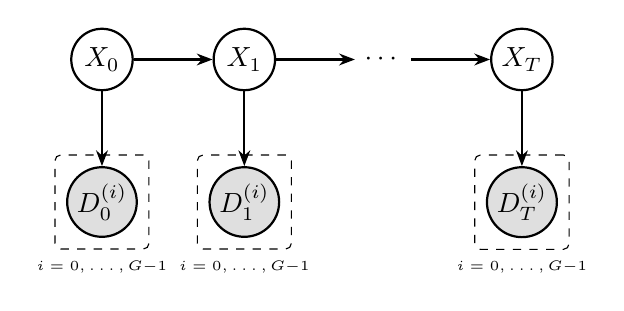
\begin{tikzpicture}[
    unobserved/.style   = {circle, draw, thick, minimum size=0.78cm, inner sep=1pt},
    observed/.style = {circle, draw, thick, fill=gray!25, minimum size=0.78cm, inner sep=1pt},
    arrow/.style    = {-{Stealth[length=2mm]}, thick},
    node distance   = 0.95cm and 1.0cm
]
\node[unobserved]                (X0)   {$X_0$};
\node[unobserved, right=of X0]   (X1)   {$X_1$};
\node[right=of X1]           (dots) {$\cdots$};
\node[unobserved, right=of dots] (XT)   {$X_T$};
\node[observed, below=of X0] (D0)   {$D_0^{(i)}$};
\node[observed, below=of X1] (D1)   {$D_1^{(i)}$};
\node[observed, below=of XT] (DT)   {$D_T^{(i)}$};
\foreach \a/\b in {X0/X1, X1/dots, dots/XT, X0/D0, X1/D1, XT/DT}
  \draw[arrow] (\a) -- (\b);
\begin{scope}[on background layer]
\foreach \n in {D0, D1, DT}
  \node[draw, dashed, rounded corners=2pt, inner sep=4pt, fit=(\n)] (p\n) {};
\end{scope}
\foreach \n in {D0, D1, DT}
  \node[font=\tiny, below=0.02cm of p\n] {$i = 0,\ldots,G{-}1$};
\end{tikzpicture}
\caption{Bayes network for the wumpus tracking model. Each unobserved $X_t$
has $G$ binary detection children.}
\label{fig:bn}
\end{figure}

\subsection{Initial-state prior}

In the absence of information about the wumpus's starting cell, a uniform
prior is used:
\begin{equation}
p(X_0 = x) = \frac{1}{G}, \qquad \forall x \in \states.
\label{eq:prior}
\end{equation}

\subsection{Transition factor}

At each step the wumpus selects a direction $d \in \{U, D, L, R\}$
uniformly and attempts a move. If the target cell is out of grid bounds the
move fails and the wumpus remains in place. Marginalising out the unobserved
direction, the transition factor is given by:

\[
p(X_{t+1} = j \given X_t = i)
\;=\;
\tfrac{1}{4} \sum_{d \in \{U, D, L, R\}}
\Ind\!\left[\,\Move(i, d) = j\,\right]
\]
where $\Move(i, d)$ returns the target cell of move $d$ from $i$, clipped
back to $i$ if the target is out of bounds.
\label{eq:transition}


\noindent The factor is sparse: each row has at most five non-zero entries
(at most four in-bounds neighbours plus the cell's own mass carried back from clipped moves).
The factor is time-homogeneous, so a single
sparse table is built at the beginning and used for every transition.

\subsection{Observation factor collapse}
\label{sec:obs}

Because every detection $D_t^{(i)}$ is observed, the $(T{+}1) G$ emission
factors can be folded into one unary factor per time step on $X_t$, removing
the detection RVs from the graph entirely. \\[8pt]
\noindent By the conditional independence of detections given the wumpus position
(Section~\ref{sec:bn}), the joint emission likelihood at time $t$
factorises as:
\begin{equation*}
p(\bd_t \given X_t = x^\star)
= \prod_{i=0}^{G-1} p \bigl(D_t^{(i)} = d_t^{(i)} \given X_t = x^\star\bigr),
\end{equation*}
and each per-cell likelihood depends only on whether cell $i$ contains the
wumpus:
\begin{equation*}
p \bigl(D_t^{(i)} = d_t^{(i)} \given X_t = x^\star\bigr) =
\begin{cases}
p_w^{d_t^{(i)}} (1{-}p_w)^{1-d_t^{(i)}} & i = x^\star, \\
p_c^{d_t^{(i)}} (1{-}p_c)^{1-d_t^{(i)}} & i \neq x^\star.
\end{cases}
\end{equation*}
Next, we can factor out the $i \neq x^\star$ terms, which do not depend on $x^\star$ and so:
\begin{equation*}
p(\bd_t \given X_t = x^\star)
= p_w^{d_t^{(x^\star)}} (1{-}p_w)^{1-d_t^{(x^\star)}}
   \cdot \overbrace{\prod_{i \neq x^\star} p_c^{d_t^{(i)}} (1{-}p_c)^{1-d_t^{(i)}}}^{ \circled{1}{-0.5pt}{0.7} } \\
\end{equation*}

Where $\circled{1}{-0.5pt}{0.7}$ is expanded to the following to enable removal of terms independent of $x^\star$:
\[
\frac{\prod_{i =0}^{G-1} p_c^{d_t^{(i)}} (1{-}p_c)^{1-d_t^{(i)}}}{p_c^{d_t^{(x^\star)}} (1{-}p_c)^{1-d_t^{(x^\star)}}}
\]
Now: 
\begin{equation*}
p(\bd_t \given X_t = x^\star) = \underbrace{\Bigl[\textstyle\prod_{i=0}^{G-1} p_c^{d_t^{(i)}}
   (1{-}p_c)^{1-d_t^{(i)}}\Bigr]}_{C_t,\;\text{independent of}\;x^\star}
\;\cdot\;
\frac{p_w^{d_t^{(x^\star)}} (1{-}p_w)^{1-d_t^{(x^\star)}}}
     {p_c^{d_t^{(x^\star)}} (1{-}p_c)^{1-d_t^{(x^\star)}}}.
\end{equation*}



$C_t$ does not depend on $x^\star$ and cancels in any posterior over $X_t$.
We define the unary observation factor:
\[
\phi_t(X_t = x^\star) \;\propto\;
\begin{cases}
p_w / p_c              & d_t^{(x^\star)} = 1, \\
(1 - p_w) / (1 - p_c)  & d_t^{(x^\star)} = 0.
\end{cases}
\]
\label{eq:phi}


\noindent This is a length-$G$ table per time step.
The $G(T{+}1)$ binary detection RVs are absent from the graph used for
inference, which becomes $T{+}1$ unobserved variables with one unary
evidence factor per step, a factor of $G$ times smaller than the naive
representation. 

\subsection{Cluster graph and inference algorithm}

The factor list (one prior, $T$ transition factors, $T{+}1$ collapsed
observation factors) is handed to \texttt{emdw}'s \texttt{ClusterGraph}
constructor with either the \texttt{LTRIP}, \texttt{BETHE} or \texttt{JTREE} construction
tag. For the chain-structured factor graph induced by this model, a non-loopy
cluster graph is constructed, so sum-product belief propagation
is exact and converges after one forward and one backward sweep.
\texttt{loopyBP\_CG} on this tree-structured CG behaves as standard
forward--backward. \\[10pt]
Sum-product marginal inference was chosen over MAP for two
reasons:\\
\begin{itemize}
  \item The per-time-step marginal $\gamma_t(x) = p(X_t \given
\bd_{0:T})$ (i.e. the posterior given all the time steps, not just the preceding ones)
 is the obvious output for visualisation and for any further
purpose of this algorithm. For example, any function that would need to know
where the wumpus is would also probably like to know how likely
the wumpus is to be there. Saying that the wumpus is in square 1 if it's only slightly less likely to be in square 2
 would be mispresenting vital information for any real world application of hunting wumpi (or wumpuses)

  \item the marginals $\gamma_t(x)$ are exactly the quantity required by the E-step of the
EM algorithm used for dataset 3 (Section~\ref{sec:em}).
\end{itemize}


\subsection{Parameter learning for unknown $p_w, p_c$ (dataset 3)}
\label{sec:em}

For dataset 3, the detection parameters are unknown. We treat them as
point estimates to be learned by the EM algorithm.
This choice keeps the graph chain-structured (so inference remains exact in
each E-step). The alternative of placing Beta priors on $p_w, p_c$ and performing full
Bayesian inference would have been possible but was not implemented because it would
have caused loopy (and thus non-exact) inference due to the parameters being shared parents of all the observation factors.

The E-step rebuilds the observation factors $\phi_t$ under the current
parameters and runs BP to give the smoothed marginals
$\gamma_t^{(k)}(x) = p(X_t = x \given \bd_{0:T}, \theta^{(k)})$. The M-step
has a closed-form solution: with $A_t = \sum_x \gamma_t^{(k)}(x)\,
d_t^{(x)}$ (the expected detection at the wumpus cell at time $t$) and
$D_t = \sum_i d_t^{(i)}$ (the total detection count at time $t$), the
updates are

\begin{equation*}
p_w^{(k+1)} = \frac{\sum_t A_t}{T+1},
\qquad
p_c^{(k+1)} = \frac{\sum_t (D_t - A_t)}{(T+1)(G-1)}.
\label{eq:mstep}
\end{equation*}

\noindent The algorithm alternates between E and M until
both of the parameters change by less than $10^{-6}$ per iteration or $50$ iterations are reached. Parameter estimates are clamped to
$[10^{-6},\, 1{-}10^{-6}]$ to avoid singular observation factors at boundary
values.\colorbox{red!100}{\ref{123}} EM is initialised at $(p_w^{(0)}, p_c^{(0)}) = (0.9, 0.1)$; 

\subsection{Scope of solution}
\label{sec:scope}

This work
addresses datasets 1--3 in depth and does not extend to datasets 4--5.
Choosing to focus on these datasets allowed for thorough analysis of datasets 1--3. 

%=========================================================
\section{Implementation}
\label{sec:impl}

The implementation comprises two main programs and a shared helper library:
\begin{itemize}
\item \texttt{miniproject.cc}: datasets 1--2 (known parameters)
\item \texttt{miniproject\_q3.cc}: dataset 3 (EM-based parameter learning)
\item \texttt{miniproject\_helpers.cc}: helper files for detection grids, ground
truth, marginals, and trajectories
\end{itemize}
Both main programs share the same skeleton: load detections, build
factors, construct cluster graph, run BP, extract per-time-step marginals,
write results to disk, but with the EM variant wrapping factor build, CG
construction, BP, and marginal extraction in an outer loop implementing the
M-step of Section~\ref{sec:em}. Each program takes the dataset directory,
output directory, initial $(p_w, p_c)$, and an optional cluster-graph type
(\texttt{LTRIP}, \texttt{JTREE} or \texttt{BETHE}) on the command line.

\subsection{Variable identifiers and shared cell domain}

Each $X_t$ is assigned a sequential integer identifier, and all $X_t$ share
a single length-$G$ cell domain instantiated once:

\begin{cppd}
vector<RVIdType> X(lastT + 1);
for (int t = 0; t <= lastT; ++t) X[t] = static_cast<RVIdType>(t);

rcptr<vector<T>> cellDom(new vector<T>(G));
for (int i = 0; i < G; ++i) (*cellDom)[i] = i;
\end{cppd}

\subsection{Building the factors}

\paragraph{Prior.} The uniform prior on $X_0$ is encoded by giving
an empty map with a default probability of $1/G$, so every
entry of the length-$G$ table is automatically $1/G$:

\begin{cppd}
map<vector<T>, FProb> emptyProbs;
rcptr<Factor> prior = uniqptr<DT>(new DT(
    {X[0]}, {cellDom}, 1.0 / static_cast<double>(G), emptyProbs));
\end{cppd}

\paragraph{Transition factor.} The transition table is built by enumerating
each source cell and moving $\tfrac{1}{4}$ of mass per direction into
the right cell. Illegal moves are mapped back to the
source cell by \texttt{clipMove}, which automatically generates the
corner/edge self-loop mass:

\begin{cppd}
auto clipMove = [W, H, &cellOf](int row, int col, int drow, int dcol) {
  int nr = row + drow, nc = col + dcol;
  if (nr < 0 || nr >= H) nr = row;
  if (nc < 0 || nc >= W) nc = col;
  return cellOf(nr, nc);
};

map<vector<T>, FProb> transProbs;
for (int i = 0; i < G; ++i) {
  const int r = rowOf(i), c = colOf(i);
  for (int d = 0; d < 4; ++d) {
    const int j = clipMove(r, c, directions[d][0], directions[d][1]);
    transProbs[{T(i), T(j)}].prob += 0.25;
  }
}
\end{cppd}

\noindent The sparse map is built once and reused across all $T$ transition
factors, using the fact that all the transitions use the same underlying structure.

\paragraph{Observation factor.} Each $\phi_t$ takes one of the two values
$\phi_{\text{on}} = p_w/p_c$ or $\phi_{\text{off}} = (1{-}p_w)/(1{-}p_c)$
per cell (see section \ref{sec:obs}), determined by the detection grid at time $t$:

\begin{cppd}
const double phiOn  = cfg.pw / cfg.pc;
const double phiOff = (1.0 - cfg.pw) / (1.0 - cfg.pc);

for (int t = 0; t <= lastT; ++t) {
  map<vector<T>, FProb> phiProbs;
  for (int row = 0; row < H; ++row)
    for (int col = 0; col < W; ++col) {
      const int j = cellOf(row, col);
      phiProbs[{T(j)}] = (detections[t][row][col] == 1) ? phiOn : phiOff;
    }
  rcptr<Factor> phi = uniqptr<DT>(new DT(
      {X[t]}, {cellDom}, defProb, phiProbs));
  factors.push_back(phi);
}
\end{cppd}

\subsection{Cluster graph and BP}

The cluster-graph construction algorithm is selectable at runtime via the command line, enabling
the \texttt{LTRIP}/\texttt{JTREE} comparison (see Section~\ref{sec:results}):

\begin{cppd}
map<RVIdType, AnyType> obsv;  
if (cfg.cgType == "JTREE")
  cgPtr = new ClusterGraph(ClusterGraph::JTREE, factors, obsv);
else if (cfg.cgType == "BETHE")
  cgPtr = new ClusterGraph(ClusterGraph::BETHE, factors, obsv);
else
  cgPtr = new ClusterGraph(ClusterGraph::LTRIP, factors, obsv);

map<Idx2, rcptr<Factor>> msgs;  MessageQueue msgQ;
unsigned nMsgs = loopyBP_CG(*cgPtr, msgs, msgQ);
\end{cppd}

\subsection{Extracting marginals and the EM loop}

For each $t$ the marginal $\gamma_t$ is obtained by querying the
cluster graph for the posterior over $X_t$ and reducing for each cell value:

\begin{cppd}
rcptr<Factor> q = queryLBP_CG(cg, msgs, {X[t]})->normalize();
for (int j = 0; j < G; ++j) {
  rcptr<Factor> reduced = q->observeAndReduce({X[t]}, {T(j)});
  gammas[t][j] = reduced->potentialAt(
      emdw::RVIds{}, emdw::RVVals{}, true);
}
\end{cppd}

\noindent In \texttt{miniproject\_q3.cc} the E-step code is wrapped in
an EM loop. After each E-step the
$A_t$ values are computed directly from \texttt{gammas[t][j]} and the detection
grid, and the M-step updates $(p_w, p_c)$ per the equation in Section~(\ref{eq:mstep}):

\begin{cppd}
double sumA = 0.0, sumDminusA = 0.0;
for (int t = 0; t <= lastT; ++t) {
  double At = 0.0;
  for (int row = 0; row < H; ++row)
    for (int col = 0; col < W; ++col)
      At += gammas[t][cellOf(row, col)] * static_cast<double>(detections[t][row][col]);
  sumA += At;
  sumDminusA += static_cast<double>(Dt[t]) - At;
}
double newPw = sumA / static_cast<double>(lastT + 1);
double newPc = sumDminusA / (static_cast<double>(lastT + 1) * static_cast<double>(G - 1));
newPw = clamp(newPw, PARAM_EPS, 1.0 - PARAM_EPS);
newPc = clamp(newPc, PARAM_EPS, 1.0 - PARAM_EPS);
\end{cppd}

\subsection{Output}

For each time step the smoothed marginal is reshaped from its length-$G$
form into a $W \times H$ matrix of probabilities and written to
\texttt{marginal\_<tt>.txt}; the per-step argmax cell forms a trajectory
file in the ground-truth coordinate format $(x, y) = (\text{col},
\text{row})$.

%=========================================================
\section{Results and analysis}
\label{sec:results}

\subsection{Evaluation methodology}

The inferred trajectory is evaluated against the provided ground truth using:
\begin{itemize}
\item \textbf{Per-step accuracy}: the fraction of time steps for which
$\argmax_x \gamma_t(x)$ equals the ground-truth cell.
\item \textbf{Mean $l_2$ cell distance}: average Euclidean distance
(in cells) between the inferred argmax cell and the ground-truth cell
across time steps.
\item \textbf{Top-k accuracy}: the fraction of time steps for which the
ground-truth cell lies in the $k$ most probable cells under $\gamma_t$,
reported for $k = 1, 3, 5$.
\end{itemize}
Qualitative evaluation uses posterior heatmaps for representative time
steps with the ground-truth cell overlaid.

\subsection{Dataset 1 (5\,$\times$\,5, $p_w{=}0.95$, $p_c{=}0.05$)}

Dataset 1 was the simplest, with a small grid, and the argmax output was the same as 
the ground truth for every timestep. See image \ref{fig:d1} for the posterior heatmaps of the first
4 frames, the posterior probability was very certain of all wumpus positions for all timesteps.
\begin{figure}[ht]
\centering
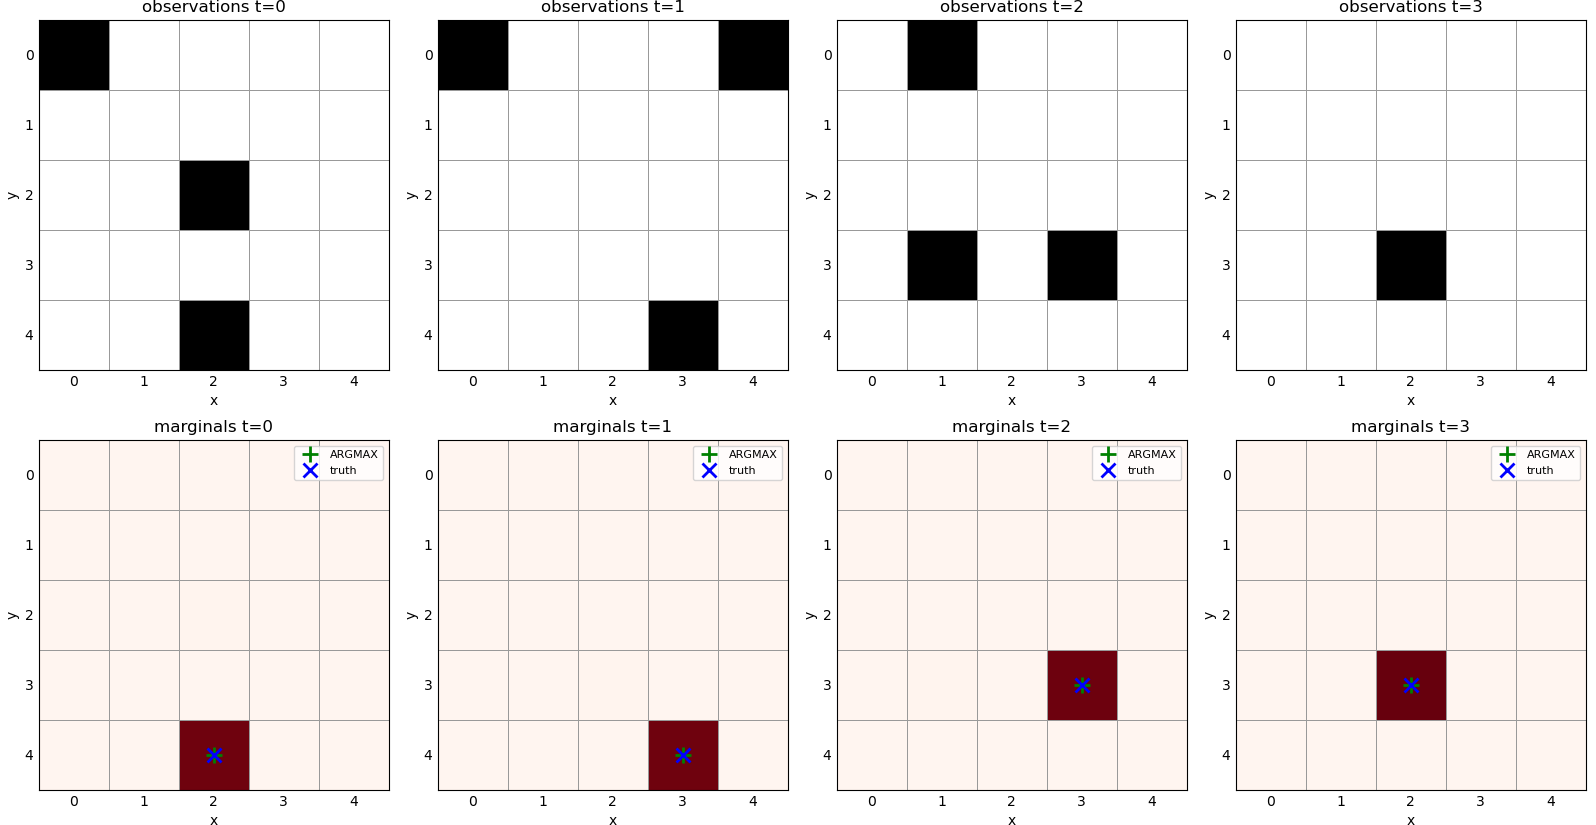
\includegraphics[width=0.95\textwidth]{output/dataset1/images/first4_sidebyside.png}
\caption{Posterior heatmaps for dataset 1 at the first 4 time steps;
ground-truth cell marked with a blue cross, the inferred argmax cell with a green cross and the
posterior probability for each cell as the heatmap.}
\label{fig:d1}
\end{figure}

\subsection{Dataset 2 (20\,$\times$\,20, $p_w{=}0.9$, $p_c{=}0.1$)}

The larger grid of dataset 2 had slightly noisier detections, but except for in cases where
2 cells were almost equally likely, the argmax was still correct. For example, in the first frame
there was not enough information to know whether the wumpus was in cell [15, 16] (p = 0.493)or [16, 17] (p = 0.487)
See figure \ref{fig:d2} for the posterior heatmaps of the first 4 frames. 

\begin{figure}[ht]
\centering
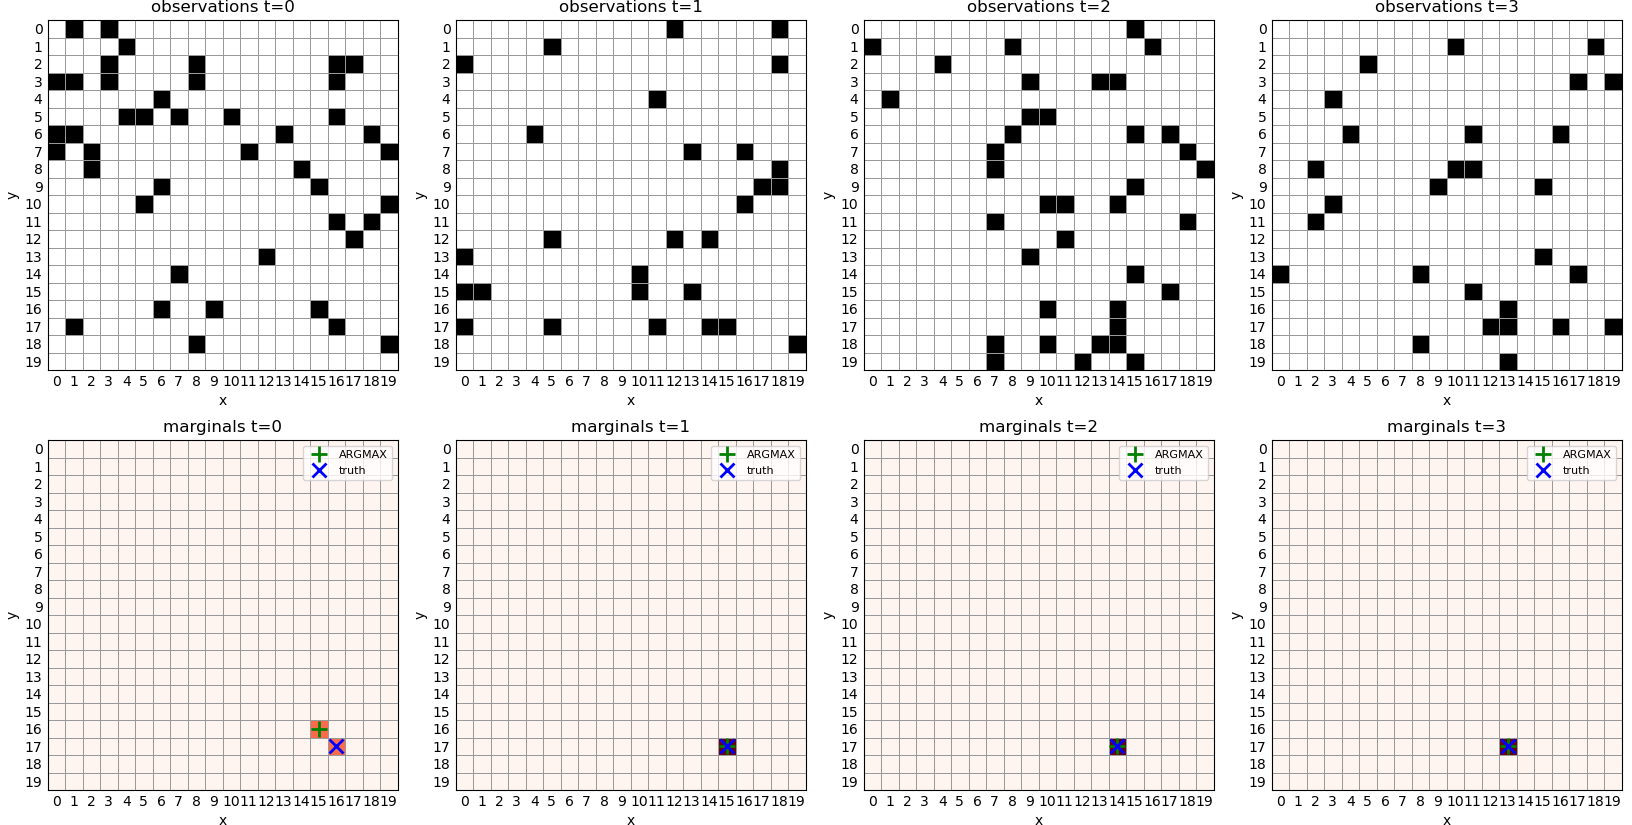
\includegraphics[width=0.95\textwidth]{output/dataset2/images/first4_sidebyside.png}
\caption{Posterior heatmaps for dataset 2 at the first 4 time steps;
ground-truth cell marked with a blue cross, the inferred argmax cell with a green cross and
the posterior probability for each cell as the heatmap.}
\label{fig:d2}
\end{figure}
\subsection{Dataset 3 (10\,$\times$\,20, EM-learned parameters)}

The accuracy on dataset 3 was the worst, however the initial observation frames were highly uninformative
due to the noisy observations being in places that the wumpus could conceivably be, and therefore the certainty in the first 
4 frames was very low and inconsistent with the ground truth. See figure \ref{fig:d3} for the posterior heatmaps of the first 6 frames.
After frame 4, the observations were more informative and the posterior certainty increased, however the argmax was still incorrect for time step 6, 
where the wumpus could have moved to 2 different positions with almost equal probability.

\begin{figure}[ht]
\centering
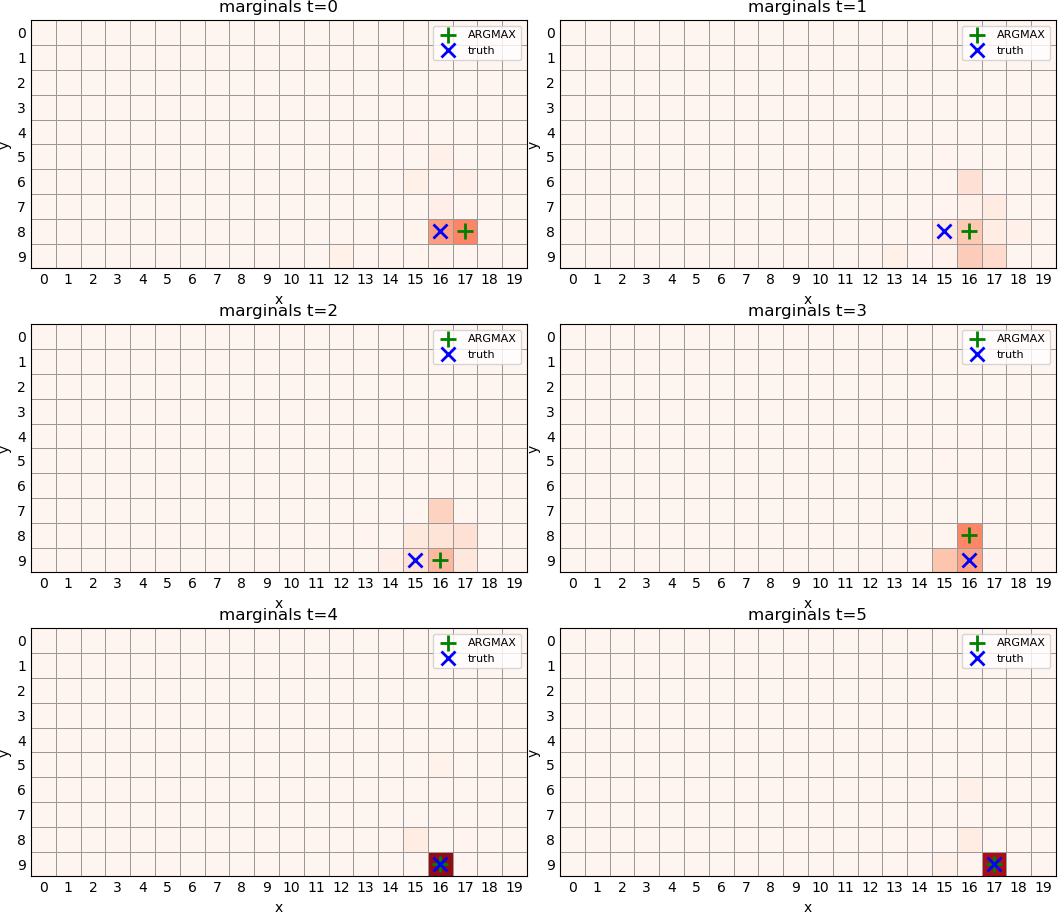
\includegraphics[width=0.95\textwidth]{images/dataset3_first6.png}
\caption{Posterior heatmaps for dataset 3 at the first 6 time steps;
ground-truth cell marked with a blue cross, the inferred argmax cell with a green cross and
the posterior probability for each cell as the heatmap.}
\label{fig:d3}
\end{figure}

\begin{table}[H]
\centering\small
\begin{tabular}{@{}lcccc@{}}
\toprule
Dataset & Per-step accuracy & Mean cell distance & Top-3 acc.\ & Top-5 acc.\ \\
\midrule
1 & 100.0\% & 0.00 & 100.0\% & 100.0\% \\
2 & 85.0\% & 0.21 & 100.0\% & 100.0\% \\
3 & 80.0\% & 0.20 & 90.0\% & 100.0\% \\
\bottomrule
\end{tabular}
\caption{Accuracy results across the three datasets.}
\label{tab:quant}
\end{table}

\begin{figure}[H]
\centering
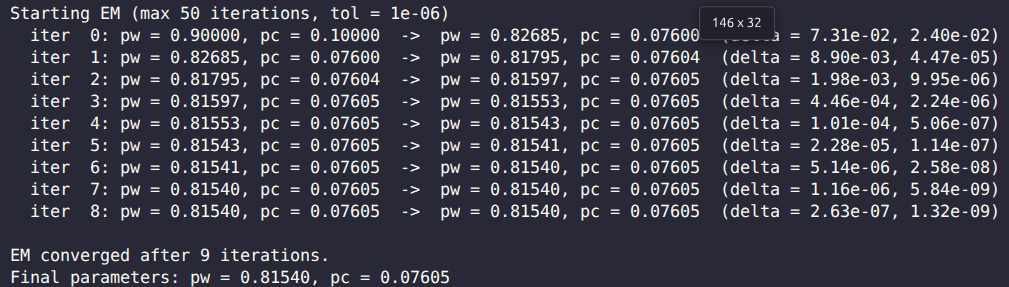
\includegraphics[width=0.6\textwidth]{images/convergence.png}
\caption{Convergence of $p_w$ and $p_c$ on dataset 3.}
\label{fig:em}
\end{figure}

EM converged after 9 iterations to $(\hat p_w, \hat p_c) = (0.815,
0.076)$ with an epsilon of $10^{-6}$

\subsection{Cluster-graph choice}

Comparing the \texttt{LTRIP}, \texttt{BETHE} and \texttt{JTREE} inference on dataset 3,
over many iterations, the mean time for \texttt{LTRIP} was lowest at 0.5s, with \texttt{JTREE} at 0.55s and \texttt{BETHE} at
0.65, all with negligible difference in time variance. In a situation where inference about the current position of the wumpus
is necessary as fast as possible, and there is a significant amount of data, \texttt{LTRIP} would be the best choice. 
If the wumpus is doing what it was originally designed for by Gregory Yob (being hunted),
faster inference of the wumpus would be more exact, because the wumpus is running away, and thus changing it's position, as it's position is being
inferred. 


%=========================================================
\section{Conclusion}

[FILL IN: brief summary paragraph. Suggested points to include:
scope (datasets 1--3); key design decisions (HMM Bayes net structure,
factor-graph collapse of detection RVs into per-step unary factors,
point-estimate EM for unknown parameters, exact sum-product BP on a chain
cluster graph); brief acknowledgement of the un-tackled extensions to
occupied cells in datasets 4--5 with an indication of the natural extension
path (loopy BP over binary map RVs vs alternating EM treating the map as a
parameter).]

The HMM-Bayes net approach was successful in inferring the wumpus position accurately most of the time, and where
it was incorrect it was incorrect but unsure of it's correctness. The EM algorithm was able to learn the parameters
for dataset 3, however the accuracy was worse than datasets 1 and 2, which is a result that would require further investigation.
The cluster graph choice did not have a significant effect on the results, however \texttt{LTRIP} was slightly faster than
\texttt{JTREE} and \texttt{BETHE}.

%=========================================================
\begin{thebibliography}{9}

\bibitem{barber2012bayesian}
D.~Barber, \emph{Bayesian Reasoning and Machine Learning}.
Cambridge University Press, 2012.

\bibitem{russell2022ai}
S.~Russell and P.~Norvig, \emph{Artificial Intelligence: A Modern Approach},
4th~ed.\ Prentice Hall, 2022.

\bibitem{koen2017rhino}
H.~Koen, H.~Roodt, and A.~De~Waal, ``An expert-driven causal model of the
rhino poaching problem,''
\emph{Ecological Modelling}, vol.~347, pp.~29--39, 2017.

\bibitem{luo2008em}
Y.~Luo, ``Basics of the EM algorithm,''
Scribe notes for COS~424: Interacting with Data (Lecturer: D.~Blei),
Lecture~11, Princeton University, Mar.~11, 2008. [Online]. Available:
\url{https://www.cs.princeton.edu/courses/archive/spr08/cos424/scribe_notes/0311.pdf}



% Add any further references you actually consulted, e.g.:
% \bibitem{koller2009pgm}
% D.~Koller and N.~Friedman, \emph{Probabilistic Graphical Models:
% Principles and Techniques}. MIT Press, 2009.

\end{thebibliography}

\end{document}